\documentclass[12pt,a4paper]{article}

\usepackage[utf8]{inputenc}
\usepackage[T1]{fontenc}
\usepackage{lmodern}
\usepackage[margin=2.5cm]{geometry}
\usepackage{booktabs}
\usepackage{tabularx}
\usepackage{array}
\usepackage{graphicx}
\usepackage{amsmath}
\usepackage{setspace}
\usepackage[hidelinks]{hyperref}
\usepackage[round,authoryear]{natbib}
\usepackage{caption}
\usepackage{longtable}
\usepackage[section]{placeins}
\captionsetup{font=small,labelfont=bf}

\newcolumntype{L}[1]{>{\raggedright\arraybackslash}p{#1}}
\onehalfspacing

\title{\textbf{Strong and Improving Fundamentals Predict Returns:\\Pre-Registered Evidence from Korean and Taiwanese Semiconductor Stocks, 2016--2026}}
\author{Matheo Witasse\thanks{EDHEC Business School, Master in Management (Data Science and AI for Business).
Every result is produced by committed code run against a pre-registration dated before the test; the decisive results
are frozen at repository tag \texttt{finding-v1}. Code, pre-registrations and results:
\url{https://github.com/matheowitasse/korea-taiwan-semiconductor-fundamentals}.}}
\date{October 2026}

\setlength{\emergencystretch}{2em}
\begin{document}
\maketitle

\begin{abstract}
\noindent We test, under a pre-registered protocol, whether firm fundamentals predict returns within the Asian
semiconductor supply chain. Ranking chip-supply-chain stocks each month on profitability and on improvement in profits
or sales predicts next-month returns in Korea: the long--short spread earns $+378$ basis points per month ($t=3.30$)
over the 2023--2026 AI boom, $+220$ bp ($t=4.06$) over 118 months since 2016, and $+158$ bp ($t=2.69$) over 74 pre-AI
months that no test had examined before it was registered. Taiwan confirms the effect on monthly revenue disclosures,
a signal with no Korean equivalent ($+212$ bp, $t=6.30$, over 127 months; $+187$ bp, $t=4.94$, before the boom). The
spread survives controls for market, size and momentum (alpha $+281$ bp in Korea, $+162$ bp in Taiwan),
market-wide Korean profitability, investment and momentum factors, Fama--MacBeth regressions and a purely rule-based
universe, and both legs contribute; book-to-price does not travel, and Japan does not clear
its pre-registered bar. The effect is sector-relative: no long-only or index-hedged construction specified in advance
demonstrates alpha, while the long--short nets $+250$ bp per month at a USD~10m fund after trading costs and breaks
even near USD~45m. Short-horizon predictability from public information is absent throughout.\\[1ex]
\noindent\textbf{Keywords:} cross-sectional returns, semiconductors, pre-registration, short-sale constraints, Korea,
Taiwan, quality, earnings momentum\\
\noindent\textbf{JEL:} G12, G14, G15
\end{abstract}

\clearpage

\section{Introduction}

Do firm fundamentals tell an investor which stocks will outperform within a single industry, and how much of that
information can be turned into returns once the costs and constraints of trading are taken into account? This paper
studies the question in the semiconductor supply chains of Korea and Taiwan between 2016 and 2026. The setting is
useful for two reasons. The fundamentals of chip companies are concentrated and frequently disclosed, and Taiwanese
firms report their revenue every month, which few markets require. The period also contains a large and well-dated
shock to the industry: Korean semiconductor exports, adjusted for working days, averaged $-2.4\%$ year-on-year growth
between structural breaks that we estimate at October 2018 and February 2024, and $+72.8\%$ after the February 2024
break, as demand for artificial-intelligence infrastructure took hold. Because the break is dated from exports rather
than from stock returns, it separates the boom from the years before it without reference to the returns we study.

The question is deliberately narrow. The paper does not propose a pricing model for Korean or Taiwanese stocks, and it
does not try to explain why the returns we document exist. It asks whether a ranking of firms on observable
fundamentals predicts the cross-section of next-month returns within the industry, whether that predictability
survives standard risk adjustment and holds outside the boom, and how much of it an investor could capture after
trading costs, short-sale rules and the availability of stock to borrow. Throughout, we call a firm attribute used to
rank stocks a \emph{characteristic} and the return on a portfolio used as a regressor a \emph{factor}; our tests are
about characteristics.

The design is pre-registered. Every hypothesis, together with its definitions and its pass/fail rule, was committed to
a version-controlled repository before the corresponding test was run, and each test was run once. In Korea, five
characteristics were tested in a discovery window covering 2023 to mid-2025, and the survivors in a validation window
that was used only after they had been fixed. Taiwan and Japan were tested as one-sided confirmations of the Korean
result, and both samples were later extended back to 2016 under separate pre-registrations. Failed tests are reported
alongside successful ones.

The main finding is that profitability and improving profits predict returns in both markets. A monthly ranking that
combines operating profitability with standardised unexpected earnings, which we call the fundamentals-improvement
signal, produces a long--short spread of $+220$ basis points per month in Korea over 118 months ($t=4.06$). The
Taiwanese analogue, based on monthly revenue growth, earns $+212$ basis points over 127 months ($t=6.30$). The effect
is present before the boom in both markets, in 74 Korean and 83 Taiwanese months that no test had examined before it
was registered ($+158$ bp, $t=2.69$, and $+187$ bp, $t=4.94$). It survives controls for the market, size and
momentum, Fama--MacBeth regressions, factors built from every listed Korean company outside the industry, and a
universe defined by industry codes alone, and both the long and the short side of the spread contribute to it.
Cheapness behaves differently: book-to-market fails validation in Korea and earns a significantly negative spread in
Taiwan. In Japan the same test is positive but does not reach its pre-registered threshold.

Two contrasts help interpret the result. The first is between ranking and timing. The same earnings information that
predicts returns as a monthly ranking produces no tradable drift around the announcements themselves: a pre-registered
test of sixty-day post-announcement drift in Korea fails narrowly in discovery and reverses sign in the following
year. The second is between the industry and the market. The top portfolio beats the equal-weight chip universe, but
the cap-weighted Korean index, which Samsung Electronics and SK Hynix dominate, returned 32\% a year over 2023--2026
against 17\% for the universe. As a result, none of the four long-only or index-hedged portfolios we specified in
advance demonstrates alpha.

The second contrast determines what can be traded. Taking short-sale eligibility from Korea's changing regulation,
borrow availability from exchange short-interest data, and costs from an explicit model of spreads, taxes, borrow fees
and market impact, the long--short strategy earns $+250$ basis points per month at a fund of USD~10m and breaks even
near USD~45m. The Korean short-selling ban of 2023--2025 does not account for the short side of the spread, which was
weaker while the ban was in force, and a direct test of the limits-to-arbitrage explanation does not support it.

The paper contributes to three strands of research. It adds evidence from one industry, in two Asian markets with
different disclosure regimes and across a technology boom, to the work showing that profitability and earnings-based
signals predict returns \citep{novymarx2013,famafrench2015,asness2019,chanjegadeeshlakonishok1996} and that return
patterns outside the United States differ from those within it \citep{rouwenhorst1999,famafrench2012,houkarolyikho2011}.
Following \citet{moskowitzgrinblatt1999}, it shows that whether such a pattern counts as alpha depends on the benchmark
against which it is measured, and it carries the analysis through to capacity under a short-selling regime that
changed three times during the sample \citep{miller1977,beberpagano2013}. Finally, it applies to an entire search the
pre-registration that \citet{harvey2017} recommends for empirical finance, as a response to the concerns about
data mining raised by \citet{harvey2016} and \citet{mcleanpontiff2016}. The search behind the result was broad, and
most of it failed: customs export releases, overnight transmission from US to Asian trading sessions, investor flows
by participant type and calendar effects show no predictability at daily frequency.

The rest of the paper is organised as follows. Section~\ref{sec:lit} reviews the related literature.
Sections~\ref{sec:data} and~\ref{sec:method} describe the data, the signals and the protocol. Section~\ref{sec:results}
reports the main result and its robustness, Section~\ref{sec:impl} asks whether it can be traded, and
Section~\ref{sec:negative} summarises the tests that failed. Sections~\ref{sec:limits} and~\ref{sec:conclusion} discuss
the limitations and conclude.

\section{Related literature}\label{sec:lit}

Studies of the cross-section of stock returns rely on two related ideas that are worth keeping apart. A factor model
explains average returns through exposure to a small number of portfolio returns. In the intertemporal model of
\citet{merton1973}, such factors arise as hedges against changes in investment opportunities, which is the theoretical
link between a portfolio whose return is priced and a variable that predicts returns. A characteristic-based test asks
instead whether a firm attribute, measured before the return, predicts which stocks earn more. \citet{danieltitman1997}
argue that for size and book-to-market it is the characteristic itself, rather than covariance with a factor, that
accounts for the return premium. Profitability has been studied in both forms. \citet{novymarx2013} shows that gross
profitability predicts the cross-section of returns about as strongly as book-to-market, \citet{famafrench2015} add a
profitability factor to their asset-pricing model, and \citet{asness2019} find that a composite measure of quality
earns a premium in many markets.

Earnings information has a long history in this literature. Prices respond to earnings news with a delay
\citep{ballbrown1968}, and the drift that follows earnings announcements is one of the most persistent anomalies
documented \citep{bernardthomas1989}. \citet{chanjegadeeshlakonishok1996} show that momentum based on earnings is
distinct from momentum based on prices and that both predict returns over the following months. In Korea,
\citet{eom2019} link post-announcement drift to individual investors who trade against earnings news.

Evidence from outside the United States is more mixed. \citet{famafrench2012} find value premia in all four regions
they study and momentum in all of them except Japan, and \citet{famafrench2017} report that the performance of their
five-factor model varies considerably across regions. In emerging markets,
\citet{rouwenhorst1999} finds return premia similar to those of developed markets but with a strongly local character,
and \citet{houkarolyikho2011} show that global returns are better described by momentum and cash-flow-to-price factors
than by size and book-to-market. This work leaves open whether an effect measured within one industry of one country is
distinct from the market-wide premia of that country.

Industry composition matters in its own right. \citet{moskowitzgrinblatt1999} show that much of the momentum in
individual stock returns reflects momentum in industries, so that the performance of a portfolio depends on whether it
is judged against the market or against its own industry. Holding the industry fixed removes that source of return but
makes the choice of benchmark central, which is one reason to study implementation alongside predictability.

The breadth of the search behind published results has itself become a subject of research. \citet{harvey2016} count
hundreds of proposed factors and argue that, once this is accounted for, a new factor should clear a $t$-statistic of
about 3.0 rather than the conventional 2.0. \citet{mcleanpontiff2016} find that the returns to published anomalies
decline after publication, and \citet{harvey2017} urges the field to adopt practices that other sciences use to
control false discoveries, pre-registration among them. Pre-registration nonetheless remains rare in empirical finance.

Short-sale constraints connect predictability to implementation. When pessimistic investors cannot sell short, prices
reflect the views of the optimists \citep{miller1977}, and arbitrage is limited by the capital and constraints of the
arbitrageurs themselves \citep{shleifervishny1997}. Bans on short selling offer natural experiments: during the
2007--09 crisis they reduced liquidity and slowed price discovery without supporting prices \citep{beberpagano2013}.
Korea changed its short-selling rules three times between 2021 and 2025, while Taiwan did not, which allows the two
markets to be compared under different constraints. Finally, prices can move ahead of scheduled macroeconomic news, as
the drift before US monetary-policy announcements documented by \citet{luccamoench2015} shows; the export releases
examined among our negative results are a regional counterpart.

\section{Data}\label{sec:data}

\begin{table}[htbp]
\centering
\caption{Samples}
\small
\begin{tabularx}{\textwidth}{l L{4.6cm} L{4.2cm} X}
\toprule
Market & Universe & Fundamentals & Sample \\
\midrule
Korea & 262 chip-supply-chain companies in 2023--2026, 285 back to 2016, \textbf{including 34 later delisted} &
DART quarterly statements; 80{,}718 filing dates & 2016-11 -- 2026-08 \\
Taiwan & 416 companies (TWSE and TPEx sector codes 24, 28), rebuilt point-in-time & Monthly revenue disclosures;
month-end valuation ratios & 2016-01 -- 2026-08 \\
Japan & 276 companies (electric appliances, precision instruments) & J-Quants quarterly statements with disclosure
timestamps & 2022-10 -- 2026-09 \\
\bottomrule
\end{tabularx}
\end{table}

Survivorship is handled differently in each market. The Korean universe includes companies delisted during the sample, reconstructed from the
exchange's delisting register and priced through their final liquidation trading, where single-day losses of $-44\%$ to
$-68\%$ occur. For Taiwan we rebuilt the universe month by month from the filing archive, whose monthly revenue files
carry each company's industry at the time, and priced it with exchange month-end quotes covering companies that have
since left the market. That exercise showed the concern is largely moot there: of 417 chip codes appearing between 2016
and 2026, 416 are still listed, and the effect is unchanged on the point-in-time universe ($+162$ bp per month,
$t=3.87$, over the pre-AI window; $+185$ bp, $t=4.49$, marking each exit at $-50\%$). The Japanese universe still
contains only currently listed companies, which removes the worst outcomes from the bottom portfolio and therefore
\emph{understates} the spread there.

To avoid look-ahead bias, a quarter's financial data enter the signal only from the day after the company's first
earnings disclosure for that quarter, which comes a median of 45 days after the quarter ends. In Japan, where
disclosure timestamps are available, statements released at or after 15:00 local time are treated as known only from
the next trading day. Prices are taken from Yahoo Finance; for the Japanese universe we compared them with official
exchange prices and found a daily return correlation of 0.9992, with level differences attributable to
dividend-adjustment conventions.

Table~\ref{tab:summary} describes the two samples behind the headline result. The
Korean cross-section holds a median of 224 stocks with a next-month return and 205 with a quality score; the typical
company is small, with a median market capitalisation of KRW~172~bn (about USD~130m) where market caps are available.
The two halves of the Korean signal are only loosely related: the median monthly cross-sectional correlation between
the quality and earnings-momentum scores is 0.20, so the combination is not one characteristic measured twice.
Earnings momentum needs eight prior quarters of profit and the DART series begin in 2015, so it is defined only from
August 2018; before that the Korean signal consists of quality alone (Section~\ref{sec:preai}).

\begin{table}[!htbp]
\centering
\caption{Summary statistics, 2016--2026. Names are the number of stocks with the variable in a month; percentiles
are across all stock-months.}
\label{tab:summary}
\footnotesize
\setlength{\tabcolsep}{4.5pt}
\begin{tabular}{lrrrrrr}
\toprule
& \multicolumn{3}{c}{Names per month} & \multicolumn{3}{c}{Distribution} \\
\cmidrule(lr){2-4}\cmidrule(lr){5-7}
Variable & Median & Min & Max & 10th pct & Median & 90th pct \\
\midrule
\textit{Korea, 2016-11 -- 2026-08} \\
Quality (TTM op.\ profit / assets) & 205 & 162 & 273 & $-0.115$ & $0.024$ & $0.136$ \\
Earnings momentum (SUE), from 2018-08 & 209 & 159 & 254 & $-1.55$ & $-0.01$ & $1.57$ \\
Next-month return & 224 & 178 & 282 & $-0.155$ & $0.000$ & $0.186$ \\
Market cap, KRW bn (2022-07 onward) & 248 & 221 & 261 & 34 & 172 & 1{,}199 \\
\addlinespace
\textit{Taiwan, 2016-02 -- 2026-08} \\
Revenue momentum ($z$-score) & 379 & 167 & 416 & $-0.60$ & $-0.10$ & $0.55$ \\
Next-month return & 375 & 342 & 416 & $-0.116$ & $0.003$ & $0.172$ \\
\bottomrule
\end{tabular}
\end{table}

\section{Method}\label{sec:method}

\subsection{Characteristics and signals}

At each month end, stocks are scored on \emph{quality} (operating profit over the trailing
four quarters divided by total assets); \emph{earnings momentum} (standardised unexpected earnings in Korea,
operating-profit growth against the same quarter a year earlier in Japan, monthly revenue growth against the same month
a year earlier in Taiwan); \emph{value} (book equity to market capitalisation); and, in the Korean discovery test only,
\emph{price momentum} (the return from twelve months to one month before formation) and \emph{size} (minus log market
capitalisation). Characteristics are ranked cross-sectionally within market and month, converted to $z$-scores
winsorised at $\pm 3$, and averaged.

Three such averages appear in the paper. The \emph{five-characteristic composite} averages all five Korean
characteristics and is the object of the Korean discovery and validation tests (Section~\ref{sec:results}). The
\emph{three-characteristic composite} averages quality, earnings momentum and value, and is the signal of the
pre-registered Japanese confirmation test. The \emph{fundamentals-improvement signal} averages quality and earnings
momentum only, or uses revenue momentum alone in Taiwan, where quality is not available; it is the headline signal of
Figure~\ref{fig:cum} and of Sections~\ref{sec:results} and~\ref{sec:impl}.

The fundamentals-improvement signal was specified after the Korean validation, in a written specification committed
before any test of it: value was dropped because it failed Korean validation and reversed sign in Taiwan, and the two
characteristics that had each passed discovery and validation were kept. Its own out-of-sample evidence is therefore
not the Korean validation window but the tests that came after it---the pre-AI extensions in both markets and live
months (Table~\ref{tab:windows}).

Formally, for stock $i$ at month end $t$, let $z_t(x_i)$ denote the cross-sectional $z$-score of
characteristic $x$, winsorised at $\pm 3$. The Korean fundamentals-improvement signal is
\begin{equation}
S_{i,t} = \tfrac{1}{2}\left[ z_t\!\left(\frac{\mathrm{OP}^{\mathrm{TTM}}_{i,t}}{A_{i,t}}\right) + z_t\!\left(\mathrm{SUE}_{i,t}\right)\right],
\label{eq:signal}
\end{equation}
where $\mathrm{OP}^{\mathrm{TTM}}$ is operating profit over the last four reported quarters, $A$ total assets, and
$\mathrm{SUE}$ the year-on-year change in quarterly operating profit scaled by the standard deviation of that change
over the previous eight quarters; when one component is missing the other is used alone. In Taiwan, $S_{i,t}$ is the
$z$-score of the latest monthly revenue against the same month a year earlier.

\subsection{Portfolios and regressions}

Stocks are sorted each month into equal-weight quintiles $Q_1,\dots,Q_5$ on
$S_{i,t}$ and held for one month. The long--short return is
\begin{equation}
R^{LS}_{t+1} = \frac{1}{|Q_5|}\sum_{i\in Q_5} r_{i,t+1} - \frac{1}{|Q_1|}\sum_{i\in Q_1} r_{i,t+1},
\label{eq:ls}
\end{equation}
and the reported statistic is its time-series mean with Newey--West standard errors (three lags). Risk-adjusted
returns are the intercept $\alpha$ of
\begin{equation}
R^{LS}_{t} = \alpha + \boldsymbol{\beta}'\mathbf{F}_t + \varepsilon_t,
\label{eq:alpha}
\end{equation}
where $\mathbf{F}_t$ holds the local index return and long--short factors built as in~\eqref{eq:ls}. Fama--MacBeth
regressions estimate, month by month,
\begin{equation}
r_{i,t+1} = a_t + b_t\, S_{i,t} + \mathbf{c}_t'\mathbf{X}_{i,t} + e_{i,t+1},
\label{eq:fm}
\end{equation}
with controls $\mathbf{X}_{i,t}$ standardised the same way, and report the mean of $b_t$ with a Newey--West $t$-statistic.
Months containing a close-to-close move greater than $31\%$---impossible under the $\pm 30\%$ daily limits, and therefore
an unadjusted corporate action---are excluded unless the stock is delisted within ten trading days.

\subsection{Protocol and inference}

Each hypothesis, its definitions and its pass/fail rules were committed to the project's
version-controlled repository before the test was run; the registrations are self-kept rather than lodged with a
third-party registry, and their order is documented by the repository history. Korea used a discovery window
(2023-01 -- 2025-06) and a validation window (2025-07 -- 2026-08) that was used only after the discovery tests had been
run and their survivors fixed. Taiwan and Japan were tested as one-sided
confirmations of the Korean hypothesis, with direction fixed in advance.

\begin{table}[htbp]
\centering
\caption{Sample windows, the signal tested in each, and its status (spreads in bp/month, $t$ in parentheses)}
\label{tab:windows}
\footnotesize
\setlength{\tabcolsep}{3.5pt}
\begin{tabularx}{\textwidth}{@{}l l r >{\raggedright\arraybackslash}p{2.7cm} >{\raggedright\arraybackslash}X l@{}}
\toprule
Window & Dates & Months & Signal & Status & Result \\
\midrule
\multicolumn{6}{@{}l}{\textit{Korea}} \\
Discovery & 2023-01--2025-06 & 30 & five-characteristic composite & discovery; Holm across six tests & $+147$ $(2.69)$ \\
Validation & 2025-07--2026-08 & 14 & survivors of discovery & untouched until survivors fixed & $+427$ $(2.03)$ \\
AI era & 2023-01--2026-08 & 44 & fundamentals-improvement & specified after validation; not itself out of sample & $+378$ $(3.30)$ \\
Pre-AI & 2016-11--2022-12 & 74 & fundamentals-improvement & pre-registered; months never examined & $+158$ $(2.69)$ \\
Full history & 2016-11--2026-08 & 118 & fundamentals-improvement & the two rows above combined & $+220$ $(4.06)$ \\
\addlinespace
\multicolumn{6}{@{}l}{\textit{Taiwan}} \\
AI era & 2023-01--2026-08 & 44 & revenue momentum & pre-registered one-sided confirmation & $+259$ $(4.08)$ \\
Pre-AI & 2016-01--2022-12 & 83 & revenue momentum & pre-registered; months never examined & $+187$ $(4.94)$ \\
Full history & 2016-01--2026-08 & 127 & revenue momentum & the two rows above combined & $+212$ $(6.30)$ \\
\addlinespace
\multicolumn{6}{@{}l}{\textit{Japan}} \\
Decisive & 2022-10--2024-06 & 21 & three-characteristic composite & pre-registered; bar $t>2$ not met & $+162$ $(1.80)$ \\
\addlinespace
\multicolumn{6}{@{}l}{\textit{Live}} \\
Korea & from 2026-09 & --- & fundamentals-improvement & out of sample, recorded monthly & pending \\
\bottomrule
\end{tabularx}
\par\smallskip\raggedright\footnotesize Korean validation, by characteristic: five-characteristic composite $+427$ $(2.03)$, quality
$+600$ $(4.43)$, earnings momentum $+604$ $(3.34)$.
\end{table}

Each pre-registered study corrects for its own multiple comparisons with the Holm procedure; no
correction is applied across the roughly ninety tests of the project as a whole. The claim therefore does not rest on
any single $p$-value but on replication in windows and a market that no earlier test had examined---the pre-AI and
Taiwanese rows of Table~\ref{tab:windows}. Table~\ref{tab:inference} lists the procedures and where each is used. Against the
stricter hurdle of $t\approx3$ proposed by \citet{harvey2016}, the full-sample spreads, risk-adjusted alphas and
Fama--MacBeth coefficients of both markets pass; the Korean discovery and validation tests of the five-characteristic
composite ($t=2.69$ and $2.03$), the long-leg alphas ($t=2.86$ and $2.27$) and the Korean pre-AI extension ($t=2.69$) do
not, and are judged against their pre-registered bar of $t>2$.

\begin{table}[htbp]
\centering
\caption{Inference procedures and where each is used}
\label{tab:inference}
\footnotesize
\begin{tabularx}{\textwidth}{@{}>{\raggedright\arraybackslash}p{4.6cm} >{\raggedright\arraybackslash}X >{\raggedright\arraybackslash}p{4.2cm}@{}}
\toprule
Procedure & What it guards against & Where it is used \\
\midrule
Newey--West standard errors, three lags & autocorrelation in monthly spreads & every reported $t$-statistic \\
Holm correction & family-wise error within one study & every pre-registered study with more than one test \\
Permutation placebo (signal shuffled across stocks within each month, 500--5{,}000 draws) & reliance on the $t$
distribution & every pre-registered test \\
Circular-shift placebo (signal series rolled against returns by a random offset) & spurious timing, keeping the
signal's own autocorrelation & the exploratory scan (Appendix~C) \\
Westfall--Young max-$t$ & the best result of a whole search looking good by chance & the exploratory scan
(Appendix~C) \\
Benjamini--Hochberg & the false-discovery rate across a search & the exploratory scan (Appendix~C) \\
\bottomrule
\end{tabularx}
\end{table}

\section{Results}\label{sec:results}

\subsection{Main result}\label{sec:main}

Table~\ref{tab:main} reports the monthly long--short spreads. In Korea, six characteristics entered discovery under a
Holm correction; the five-characteristic composite, value, quality and earnings momentum passed, and price momentum and size did
not. Of the four survivors, three were confirmed in the untouched validation window---the five-characteristic composite at
$+427$ bp per month ($t=2.03$, placebo $p=0.002$), quality at $+600$ bp ($t=4.43$) and earnings momentum at $+604$ bp
($t=3.34$)---while value was not ($t=1.39$).

The fundamentals-improvement signal combines the two characteristics that were confirmed individually. Over the 44
months of 2023--2026 it earns $+378$ bp per month in Korea ($t=3.30$), and the spread is positive in 75\% of months.
Taiwan, tested as a one-sided confirmation on revenue momentum, earns $+259$ bp ($t=4.08$, placebo $p<0.001$), positive
in 70\% of months. Book-to-price behaves differently in the two markets: it fails validation in Korea and is
significantly negative in Taiwan ($-146$ bp, $t=-2.09$), so the result is about improvement rather than cheapness.
Figure~\ref{fig:cum} shows the cumulative spread over the full samples, including the pre-AI years examined in
Section~\ref{sec:preai}.

\begin{table}[!htbp]
\centering
\caption{Monthly long--short spreads (basis points, $t$-statistics in parentheses). The 44-month Korean row uses the
fundamentals-improvement signal, specified after the validation window; its out-of-sample tests are in
Section~\ref{sec:preai}. Taiwan's signal throughout is revenue momentum.}
\label{tab:main}
\small
\begin{tabularx}{\textwidth}{@{}>{\raggedright\arraybackslash}X c c@{}}
\toprule
& Korea & Taiwan \\
\midrule
Discovery, 30 months: five-characteristic composite & $+147$ $(2.69)$ & --- \\
Validation, 14 months: five-characteristic composite & $\mathbf{+427}$ $(2.03)$ & --- \\
Validation: quality & $+600$ $(4.43)$ & n/a \\
Validation: earnings momentum & $+604$ $(3.34)$ & --- \\
2023--2026, 44 months: fundamentals-improvement & $+378$ $(3.30)$ & $\mathbf{+259}$ $(4.08)$ \\
Value & not confirmed $(1.39)$ & $-146$ $(-2.09)$ \\
\bottomrule
\end{tabularx}
\end{table}

\begin{figure}[!htbp]
\centering
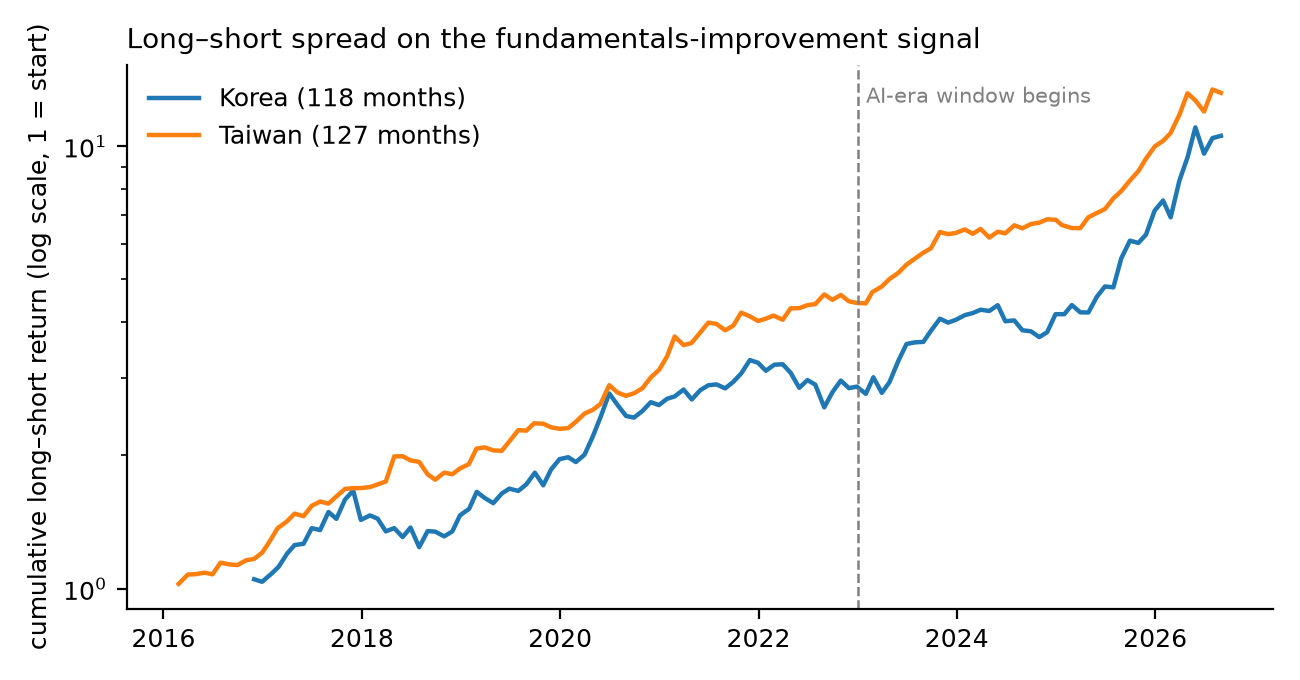
\includegraphics[width=\textwidth]{figures/fig1_cumulative.png}
\caption{Cumulative long--short return on the fundamentals-improvement signal, Korea (118 months) and Taiwan
(127 months), log scale, each rebased to 1 at its own first month. The dashed line marks the start of the AI-era
window (January 2023); everything to its left is the pre-AI extension tested in Section~\ref{sec:preai}---74 months
for Korea and 83 for Taiwan, none examined before its test was run.}
\label{fig:cum}
\end{figure}

\subsection{Risk adjustment}\label{sec:risk}

Because the universe is a single sector, the natural controls are the local market and the two characteristics most
easily confused with the signal: size and past returns. We regress the monthly spread on the local index (the KOSPI
Composite in Korea, TAIEX in Taiwan) and on size and momentum spreads built inside the same universe, with Newey--West
standard errors. The alpha is $+281$ bp per month in Korea ($t=3.60$) and $+162$ bp in Taiwan ($t=3.62$)
(Table~\ref{tab:risk}). The Korean spread carries no momentum exposure ($\beta=0.01$) and a negative size loading
($-0.47$): it tilts toward the larger companies in the sector, so it is not a small-cap effect in disguise. In Taiwan,
revenue momentum and price momentum are correlated, the momentum loading is larger ($0.42$), and the alpha is
correspondingly further below the raw spread.

\begin{table}[!htbp]
\centering
\caption{Risk adjustment: the monthly spread regressed on the local index and on size and momentum spreads built inside
the same universe (Newey--West, three lags)}
\label{tab:risk}
\small
\begin{tabular}{lcccc}
\toprule
& Alpha (bp/month) & $t$ & Momentum beta & Size beta \\
\midrule
Korea  & $+281$ & $3.60$ & $0.01$ & $-0.47$ \\
Taiwan & $+162$ & $3.62$ & $0.42$ & --- \\
\bottomrule
\end{tabular}
\end{table}

\subsection{Where the spread comes from}\label{sec:legs}

We split the spread into a long leg (top quintile minus the equal-weight universe) and a short leg (the universe minus
the bottom quintile). Both earn significant risk-adjusted returns in both markets (Table~\ref{tab:legs}). In Korea they
contribute almost equally (52\% and 48\% of the spread); in Taiwan the short leg carries more of it (62\%). The short
leg is also the steadier of the two: positive in 77\% of months in both markets, and still positive in 2024, when the
long leg's contribution fell to near zero. The result is therefore neither a matter of avoiding the worst companies
alone nor of picking the best.

\begin{table}[!htbp]
\centering
\caption{Decomposition into legs (risk-adjusted alpha in parentheses)}
\label{tab:legs}
\small
\begin{tabular}{lcc}
\toprule
& Long leg (top $-$ universe) & Short leg (universe $-$ bottom) \\
\midrule
Korea  & $+196$ bp, $t=2.85$ $(+137$ bp, $t=2.86)$ & $+182$ bp, $t=3.75$ $(+144$ bp, $t=4.20)$ \\
Taiwan & $+98$ bp, $t=2.60$ $(+64$ bp, $t=2.27)$  & $+162$ bp, $t=3.57$ $(+98$ bp, $t=3.59)$ \\
\bottomrule
\end{tabular}
\end{table}

\subsection{Regression evidence and further controls}\label{sec:fm}

Portfolio sorts can be driven by a handful of extreme stocks, and a single-sector universe invites the question of
whether the result comes from how that sector was drawn. We pre-registered four further tests against those
concerns, each with a bar of $t>2$ and a Holm correction across the four; all four pass with Holm $p<0.001$
(Table~\ref{tab:fm}).

The Fama--MacBeth coefficient on the signal is $+73$ bp of next-month return per cross-sectional standard deviation in
Korea ($t=4.08$, 118 months) and $+80$ bp in Taiwan ($t=6.42$, 127 months), controlling for twelve-month momentum and
the prior month's return, neither of which carries a significant coefficient. Over the shorter windows where the
data allow size and book-to-market controls the signal remains significant ($t=3.17$ in Korea from 2022-07,
$t=3.34$ in Taiwan on exchange-listed names). One result there qualifies the sort-based evidence on value: in the
Korean regression with size, book-to-market carries a positive coefficient ($+124$ bp, $t=2.61$, 50 months), so
cheapness is not irrelevant in Korea even though it failed the pre-registered sort-based validation.

To ask whether the Korean spread is a market-wide premium in disguise, we built profitability, investment and
momentum factors from every listed Korean company outside the chip universe---a median of about 1{,}640 companies a
month---and added them to the index and in-universe momentum controls. The alpha is $+179$ bp per month ($t=4.66$)
over 2016-12 to 2026-08, against $+168$ bp ($t=4.21$) without them; none of the three factors absorbs the spread.
Finally, four of the 285 Korean companies entered the universe by name rather than by industry code (Samsung
Electronics, ISC, Wonik IPS and Jusung Engineering). Removing them changes the full-sample spread from $+220$ bp to
$+218$ bp ($t=4.01$).

\begin{table}[!htbp]
\centering
\caption{Regression evidence and further controls (pre-registered; bar $t>2$, Holm across F1, F2, A1 and U1).
Fama--MacBeth coefficients are bp of next-month return per cross-sectional standard deviation.}
\label{tab:fm}
\small
\begin{tabularx}{\textwidth}{@{}>{\raggedright\arraybackslash}X l r r r@{}}
\toprule
Test & Window & Months & Estimate & $t$ \\
\midrule
F1 Fama--MacBeth, Korea (controls: momentum, reversal) & 2016-11 -- 2026-08 & 118 & $+73$ & 4.08 \\
F2 Fama--MacBeth, Taiwan (same controls) & 2016-02 -- 2026-08 & 127 & $+80$ & 6.42 \\
A1 Korean alpha with market-wide profitability, investment and momentum factors & 2016-12 -- 2026-08 & 113 & $+179$ & 4.66 \\
U1 Korean spread, rule-only universe (281 of 285 companies) & 2016-11 -- 2026-08 & 118 & $+218$ & 4.01 \\
\addlinespace
\multicolumn{5}{@{}l}{\textit{Secondary (shorter windows)}} \\
F3 Fama--MacBeth, Korea, adding size and book-to-market & 2022-07 -- 2026-08 & 50 & $+99$ & 3.17 \\
F4 Fama--MacBeth, Taiwan, adding book-to-market (TWSE names) & 2016-02 -- 2026-08 & 92 & $+63$ & 3.34 \\
\addlinespace
\multicolumn{5}{@{}l}{\textit{Descriptive}} \\
Skip a month (signal at $t$, return $t{+}1 \to t{+}2$), Korea & 2016-11 -- 2026-08 & 117 & $+182$ & 3.57 \\
Skip a month, Taiwan & 2016-02 -- 2026-08 & 126 & $+207$ & 4.93 \\
\bottomrule
\end{tabularx}
\end{table}

The information is also slow to decay. Skipping a month between formation and holding leaves $+182$ bp in Korea and
$+207$ bp in Taiwan, so the spread is not a first-month microstructure effect. Over the full samples the long--short
has an annualised Sharpe ratio of 1.23 in Korea (maximum drawdown $-25.5\%$, positive in 64\% of months) and 1.96 in
Taiwan (maximum drawdown $-11.5\%$, 69\%). The weakest Korean years are 2018 ($+34$ bp a month), 2022 ($-88$ bp) and
2024 ($+34$ bp); Taiwan has no negative calendar year.

\subsection{Does the effect predate the AI boom?}\label{sec:preai}

The main result covers 44 months inside one semiconductor upcycle, and the natural objection is that it describes the
boom rather than the market. We pre-registered an extension of the Korean sample to the earliest date the data allow,
fixing in advance that a failure would narrow the paper's claim to a regime-specific effect.

Three additions were needed: delisting records back to 2015 from the exchange register (716 delistings, 34 of them in
the chip universe, against 11 in the original sample), daily prices for those delisted companies, and DART fundamentals
back to 2015. Because the multi-account interface returns only annual figures for 2015, trailing-four-quarter signals
begin in November 2016; that date is set by data availability, not chosen.

Over \textbf{2016-11 to 2022-12---74 months, a median of 188 names, none of it examined before this test---the
long--short spread is $+158$ bp per month ($t=2.69$, one-sided placebo $p<0.001$)}. Controlling for the index and a
momentum spread leaves an alpha of $+121$ bp ($t=2.73$); the size control is unavailable before the 2022-06
market-capitalisation snapshot, so those regressions use two controls rather than three. Over the full 118 months the
spread is $+220$ bp ($t=4.06$).

One qualification applies to the start of this window. Earnings momentum needs eight prior quarters and the DART
series begin in 2015, so no stock has a SUE score before August 2018: the first 21 months test quality alone. That
stretch earns $+123$ bp ($t=0.91$); over the 53 pre-AI months in which both components are defined (2018-08 to
2022-12) the combined signal earns $+172$ bp ($t=2.69$), and over all 97 such months to 2026-08, $+241$ bp
($t=4.08$). The split was not pre-registered; it follows from a data-coverage check made while preparing
Table~\ref{tab:summary} and is reported as such.

The Taiwanese archive also reaches back to 2016, so the same design was repeated there and pre-registered before any pre-2022 Taiwanese data was downloaded. Over \textbf{2016-01 to 2022-12---83 usable months, a median of 367 scored names---revenue momentum earns $+187$ bp per month ($t=4.94$, placebo $p<0.001$)}, with a risk-adjusted alpha of $+183$ bp ($t=6.60$) against the local index and a momentum spread. Over the full 2016--2026 Taiwanese sample (127 months) the spread is $+212$ bp ($t=6.30$). Book-to-price is flat over the same unseen window ($+0.7$ bp, $t=0.03$) before turning negative in the AI era, so the contrast between improvement and cheapness is not a property of the boom either.

Descriptively, the effect is weaker outside the boom and never absent: $+196$ bp per month in 2017--2019, $+146$ bp
through the 2018--19 memory downturn, $+119$ bp in 2020--2022 and $+325$ bp in 2023--2026. We report these sub-periods
without significance tests and did not re-cut the sample after seeing them.

\subsection{Is it illiquidity?}

The universe is small and mid-cap, so the first alternative explanation is that equal-weight quintiles in illiquid names
manufacture spreads through trading frictions rather than information. We specified the test before running it. Sorting
the universe each month into terciles of Amihud illiquidity (trailing twelve months) and computing the spread
\emph{inside} each tercile gives $+310$ bp per month in the most liquid third ($t=2.24$), $+409$ bp in the middle
($t=2.96$) and $+303$ bp in the least liquid third ($t=2.40$). The effect is not concentrated where trading is hardest.
Adding an illiquidity factor, built as a long--short of the Amihud rank in the same universe, to the market, size and
momentum controls leaves the alpha at $+252$ bp per month ($t=3.69$), against $+281$ bp ($t=3.60$) without it. Excluding
the smallest 20\% of the universe by market capitalisation gives $+385$ bp ($t=3.08$); excluding stocks priced below
KRW~1{,}000 gives $+365$ bp ($t=3.26$).

Value-weighting is the one screen that weakens the result: $+517$ bp per month with $t=1.91$ over the 44 months, and
$+67$ bp ($t=0.55$) for the five-characteristic composite in the 30-month discovery window. The point estimate is large and the
significance is not there; with 44 months we treat this as inconclusive rather than as evidence of absence, and note
that value-weighting in a universe whose largest constituents are Samsung Electronics and SK Hynix mostly measures those
two companies.

\subsection{Is it just the Korean quality premium?}\label{sec:qualitycontrol}

Profitability and quality premia are documented in many markets, including a 24-country study that covers Korea
\citep{asness2019}, so the natural question is whether our result is that premium appearing inside one sector. No
off-the-shelf benchmark exists: AQR's country files and Ken French's international library both stop at developed
markets and exclude Korea. We therefore built one.

KOR-QMJ ranks every KOSPI- and KOSDAQ-listed company in the DART register on the same quality measure we
use---trailing-four-quarter operating profit over total assets---and takes the equal-weight quintile spread, a median of
1{,}807 companies a month from December 2016. The decisive version, KOR-QMJ-ex-chip, excludes the 285 companies of our
universe so that the control does not contain the stocks being explained.

Adding it to the market, size and momentum controls leaves the chip-sector alpha at \textbf{$+285$ bp per month
($t=3.78$)}, against $+281$ bp ($t=3.60$) without it; over the extended window the figures are $+263$ bp ($t=3.85$). The
loading on the market-wide factor is positive but small ($0.32$, $t=2.22$) and raises the regression's $R^2$ by four
points.

The reason the control changes so little is worth stating plainly: \textbf{the market-wide Korean quality premium is
absent in this period.} KOR-QMJ earns $+12.6$ bp per month ($t=0.29$) over the 44 months of the AI-era sample and
$-6.8$ bp ($t=-0.13$) excluding chip names, and its correlation with the chip spread is $0.27$. The effect we document
is sector-specific; there is no Korea-wide premium for it to be an instance of.

Two caveats travel with this. KOR-QMJ uses one accounting definition of quality, where the literature uses composites;
and it is built from companies listed today, so it is survivorship-biased upward---which makes it a conservative
control, since a stronger market-wide factor would absorb more of the chip spread, not less.

\subsection{Japan: not confirmed}\label{sec:japan}

Japan's unseen window (2022-10 -- 2024-06, 21 usable months, containing the 2022--23 memory downturn) gives $+162$ bp per month on the three-characteristic composite, $t=1.80$, against a pre-registered bar of $t>2$: \textbf{not confirmed}. In that window the strongest characteristic was
value ($+263$ bp, $t=3.93$), the opposite of the Taiwanese result. We report this as a hypothesis---that value performs
in downturns while improvement signals perform in upcycles---not as a finding.

\section{Implementability: eligibility, borrow and capacity}\label{sec:impl}

A cross-sectional spread is not a strategy. This section asks what an investor could actually run, and answers it in
three steps: may these stocks be sold short, is there anything to borrow, and what is left after costs.

\subsection{Eligibility}

Korean short selling passed through four regimes in and around our sample: a COVID-era ban (2020-03 to 2021-05); a
partial resumption in which \textbf{only KOSPI~200 and KOSDAQ~150 constituents} could be sold short (2021-05 to
2023-11-05); a second full ban (2023-11-06 to 2025-03-30); and \textbf{full resumption across all listed stocks from
2025-03-31}. Eligibility therefore binds for the first ten months of our sample, removes the short leg entirely for
seventeen, and does not bind at all for the final seventeen.

Using end-of-quarter market capitalisation to approximate index membership, a median of four of the forty-seven
bottom-quintile names per month---about 8\%---fall inside KOSPI~200 or KOSDAQ~150. That was the shortable share while
the index restriction applied. Applying eligibility by regime rather than uniformly, the short leg is tradable in
\textbf{25 of the 44 months} and earns \textbf{$+282$ bp per month ($t=4.97$), with an alpha of $+217$ bp ($t=4.36$)}
after the market, size and momentum controls. Combined with the long leg over the same months the spread is $+592$ bp
(alpha $+430$ bp, $t=4.25$).

\subsection{Is there anything to borrow?}

Eligibility is necessary but not sufficient: a stock that may be shorted still needs lendable supply. We take this from
the exchange rather than assuming it. On 17 September 2026, of the fifty names in the strategy's short side,
\textbf{76\% had short-sale volume that day} (median 1.5\% of their turnover) and \textbf{56\% carried a reported net
short position}, with a median size of \textbf{0.55\% of market capitalisation}---marginally larger than the 0.54\% of
the 350 biggest listed companies. Across four snapshots between June 2025 and September 2026 the share carrying a net
short position is stable at 56--60\%.

These shares are unremarkable, and that is the point. Across all 2,762 listed issues the same day, 79\% had short-sale
volume and 62\% carried a net short position; the rest of the chip universe was higher still, at 87\% and 72\%. The
names the strategy would short are therefore shorted slightly \emph{less} than the average Korean stock, not more, so
the short leg is neither obstructed by an absence of lendable supply nor a crowded position exposed to a squeeze. The
long side is the heavily shorted one, at 98\% and 92\% respectively---a reminder that short interest here tracks size
and liquidity rather than the signal. Two caveats apply to both measures: short-sale volume is a single day's flow, so
a borrowable name that simply was not shorted that day does not appear, and reported net short positions appear only
above the KRX disclosure threshold---0.01\% of issued shares with a KRW~100m minimum, or KRW~1bn outright, since
1~December 2024. Both figures are therefore lower bounds on what can be borrowed.

\subsection{What costs leave behind}\label{sec:costs}

We model costs per stock-month: half the bid--ask spread estimated from daily highs and lows
\citep[][median 32 bp on the long leg, 36 bp on the short]{corwinschultz2012}, 5 bp commission each way, a 20 bp
securities transaction tax on sales, a borrow fee of 1--5\% a year on the short leg, and market impact in the Amihud
form \citep{amihud2002} scaled by fund size. Monthly turnover is 18\% on the long leg and 15\% on the short.
The Korean transaction tax was 0.20\% in 2023, 0.18\% in 2024, 0.15\% in 2025 and 0.20\% again from
1~January 2026; we hold it at the 2023 and 2026 rate of 20 bp throughout, which overstates the cost by under
1 bp a month in the two intervening years.

\begin{table}[h]
\centering
\caption{Cost build-up, USD 10m fund, 3\% borrow fee}
\begin{tabular}{lrr}
\toprule
Step & Net spread (bp/month) & $t$ \\
\midrule
Gross & 378 & 3.30 \\
+ half spread & 356 & 3.13 \\
+ commission & 353 & 3.10 \\
+ securities transaction tax & 346 & 3.04 \\
+ borrow fee & 321 & 2.82 \\
+ market impact & \textbf{250} & \textbf{2.24} \\
\bottomrule
\end{tabular}
\end{table}

Net alpha after the same controls is $+155$ bp ($t=2.15$). The result is therefore \textbf{implementable, but small}: at
USD~1m the net spread is $+314$ bp (alpha $t=2.85$), at USD~10m $+250$ bp (alpha $t=2.15$), at USD~50m $-36$ bp, and the
break-even size is roughly \textbf{USD~43--47m} for the long--short and USD~57m for the long leg alone. Capacity is
bounded twice over---by impact in stocks whose median market capitalisation is KRW~90--160~bn, and by the borrow
measured above, where typical short positions are 0.55\% of a company's value.

The borrow fee is the only one of these inputs that cannot be looked up. Commissions and the transaction tax are
published, half-spreads are estimated from public prices and impact is a model, but stock-loan rates are bilateral
and have no public tape. Rather than assume a better number we report the bound. Sweeping the fee from zero to
60\% a year and holding everything else fixed, the net spread at a USD~10m fund reaches zero only at a borrow cost
of \textbf{33\% a year}, and at a USD~1m fund at \textbf{41\%}---deep special-rate territory, so the point
estimate is robust to the assumption. Statistical significance is the fragile part: the risk-adjusted alpha loses
its $t=2$ at a fee of \textbf{4.3\%} at USD~10m, and 10.8\% at USD~1m. What the borrow assumption buys is
therefore the confidence interval around the after-cost result rather than the result itself, and a reader who
believes these names are hard to borrow should read the after-cost alphas as suggestive rather than significant.

\begin{figure}[h]
\centering
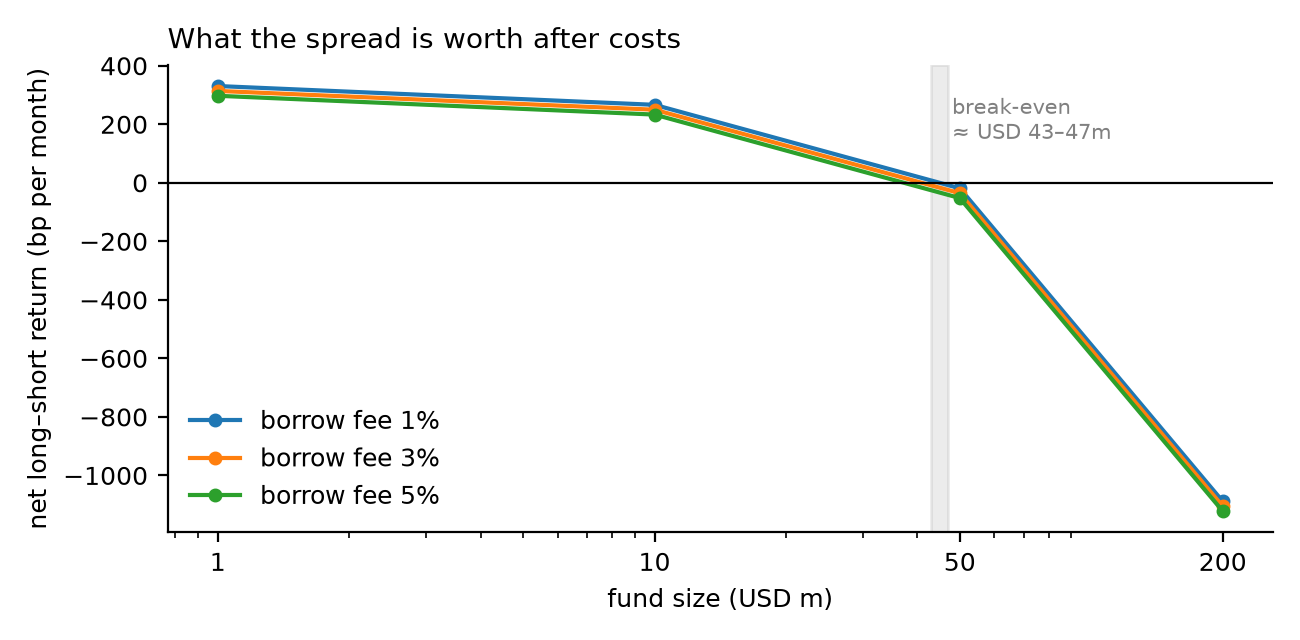
\includegraphics[width=\textwidth]{figures/fig2_capacity.png}
\caption{Net long--short return by fund size and borrow fee, after spreads, commission, transaction tax and market
impact. Break-even is roughly USD~43--47m.}
\end{figure}

Long-only constructions remain the weak case. Four were specified in advance---a 20-stock top-quintile portfolio, a
portfolio excluding the bottom 40\%, a momentum-neutral selection and an index-futures hedge---and none demonstrates
alpha ($t$ between $0.13$ and $1.37$), because the effect is \emph{sector-relative}: the signal beats the equal-weight
universe, but the cap-weighted index returned 32.0\% a year against the universe's 17.0\%, so index futures hedge the
wrong exposure. With an information ratio near $0.5$, a long-only version would need roughly sixteen years to establish
alpha.

\subsection{The short-selling ban is not the explanation}\label{sec:ban}

The 2023--25 ban covers seventeen of our forty-four months, which raises the possibility that the short-leg premium is
an artefact of the ban in the sense of \citet{miller1977}. It is not: the Korean short leg earned $+91$ bp per month
during the ban against $+234$ bp in other months, and Taiwan, which had no ban, shows the same pattern ($+35$ bp against
$+234$ bp). Both legs in both markets were weak in that window, which dates it to the 2024 factor drawdown rather than
to Korean regulation. The post-ban window is the strongest sub-period in our sample (short leg $+286$ bp, alpha
$t=3.57$).

\subsection{Limits to arbitrage: tested, not supported}\label{sec:loa}

We pre-registered a direct test of the limits-to-arbitrage explanation---that the effect survives \emph{because} the
expected losers are costly or difficult to short. In a panel of stock-months with month fixed effects, the interaction between signal rank and
index membership is $-47$ bp ($t=-0.21$; $-240$ bp, $t=-0.89$ with size controls), far from the one-sided 5\% bar.
Spreads computed inside each group point the predicted way ($+331$ bp per month, $t=3.48$ among non-members against
$+220$ bp, $t=1.26$ among members) but are not statistically distinguishable, and the member group contains only about
forty names a month. Given the short-interest evidence above, the split is better read as a size split than as a
shortability split. \textbf{We report the constraint as measured and do not claim that unshortability explains the
effect's survival.}

\section{What does not work}\label{sec:negative}

Short-horizon predictability is absent across every hypothesis we pre-registered: customs export-release surprises
predicting US or Korean semiconductor returns at one to twenty days; pre-release drift and release-day premia;
overnight US-to-Asia transmission beyond the opening price; supplier rebounds after large US declines in three markets;
investor flows by participant type; option expiry and turn-of-month effects; cross-sectional weekly reversal;
post-earnings-announcement drift at the event level \citep[for the Korean drift literature see][]{eom2019}; and drift
after dilution filings---convertible bonds and rights issues, 113 to 148 events per test. Appendix~B lists every test
with its statistic and outcome.

Two episodes are worth singling out because they bound how much the protocol matters. Post-earnings drift was the
closest this project came to a second result---a narrow failure in discovery ($+5.6\%$, $t=1.63$) that reversed sign on
the next twelve months of events---and an exploratory scan of 264 combinations produced apparent winners that a
correction for the size of the search eliminated entirely. Both are documented in Appendix~C.

\section{Limitations}\label{sec:limits}

The study has several limitations. Its scope is a single industry dominated by small and mid-sized companies, and the
semiconductor supply chain is defined through industry classifications that differ across the three markets. The
AI-era windows cover 44 months and the Korean validation window only 14. The evidence outside the boom rests on
extensions that span one memory-chip cycle in each of Korea and Taiwan, Japan's 21-month window did not confirm the
result, and live months therefore remain the only fully prospective evidence.

The data have their own weaknesses. Financial statements are current values that include restatements, so the signal
is not strictly point-in-time. Korean earnings momentum is defined only from August 2018, and market capitalisations
are unavailable before 2022 in Korea and absent in Taiwan, which confines value-weighted results and size controls to
the recent window. The Japanese universe excludes delisted companies. Family-wise error is controlled within each study
but not across the roughly ninety tests of the project or the exploratory scan of Appendix~C, so the claim rests on
replication in windows and a market that no earlier test had examined rather than on any single $p$-value.

Finally, the implementation results depend on modelled rather than observed costs. Spreads are estimated from daily
highs and lows, market impact is assumed to be linear, the transaction tax is held constant, index membership is
approximated by market capitalisation, and Korean price limits and the uptick rule are ignored. Borrow fees have no
public source; Section~\ref{sec:costs} bounds them instead of assuming a value, and shows that the net spread survives
any fee below about 33\% a year at USD~10m but loses its statistical significance above about 4.3\%.

\section{Conclusion}\label{sec:conclusion}

In a sector and a period with an unusually strong common fundamental shock, short-horizon predictability from public
information is absent, while a simple characteristic-based ranking---profitable companies whose profits or sales are
improving---predicts monthly cross-sectional returns in two independent markets. It survives standard risk
controls, market-wide factors and Fama--MacBeth regressions, and it is present before the AI boom in both markets.
Cheapness does not travel: it fails validation in Korea and reverses in Taiwan.

Whether it is investable depends on size. The long--short form survives our cost model at USD~1--10m and breaks even near USD~45m, and its
significance at USD~10m holds only while borrow costs stay below about 4\% a year; the stocks it would short are
eligible and are demonstrably shorted by others; and no pre-specified long-only construction demonstrates alpha,
because the effect is sector-relative and index futures hedge the wrong exposure. The signal is therefore
potentially implementable as a small-capacity long--short strategy, but it is not established as a scalable
long-only or index-hedged product. What is \emph{not} established is why the effect survives. The obvious candidate---that arbitrage is constrained because the expected losers are costly or
difficult to short---predicts a stronger short leg when shorting is restricted. The short leg was weaker during
Korea's ban, so we report the failed test rather than the appealing story.

Two things would sharpen the picture: a longer Japanese sample, since its decisive window is only 21 months while the Korean and
Taiwanese pre-AI windows both cover the 2018--19 memory cycle; and live out-of-sample months, which began on 21 September 2026 and are
recorded monthly.

\section*{Declarations}

\paragraph{Data availability.} Prices are from Yahoo Finance, the Korea Exchange (KRX), the Taiwan Stock Exchange and
the Taipei Exchange; financial statements from DART (Korea), the Market Observation Post System (Taiwan) and J-Quants
(Japan). The code, every pre-registration and all derived results are available at
\url{https://github.com/matheowitasse/korea-taiwan-semiconductor-fundamentals}. KRX and J-Quants data cannot be redistributed under their terms of use; the repository contains the scripts
that download them.

\paragraph{Funding.} This research received no external funding.

\paragraph{Competing interests.} None.

\bibliographystyle{chicago}
\bibliography{references}

\appendix
\section{Pre-registrations and code}
Each study's pre-registration, script and result is committed, with the pre-registration preceding the script and the
script preceding the result in the repository history. Decisive results are frozen at tag \texttt{finding-v1}.

\clearpage
\section{Full list of tests}\label{app:tests}

Every study in the project, compiled from its dated pre-registrations and results. Decisive tests carried a pre-registered pass/fail
rule; the other rows are robustness checks, diagnostics or exploratory runs, labelled as such when they were run.
Spreads are in basis points per month unless stated.

\begingroup
\footnotesize
\setlength{\tabcolsep}{3.5pt}
\begin{longtable}{@{}L{1.3cm} L{4.4cm} L{2.6cm} L{4.6cm} L{2.0cm}@{}}
\toprule
Study & Question & Market, sample & Result & Outcome \\
\midrule
\endfirsthead
\toprule
Study & Question & Market, sample & Result & Outcome \\
\midrule
\endhead
\bottomrule
\endfoot
\multicolumn{5}{@{}l}{\textit{B.1 Short-horizon predictability}} \\
Q1 & Customs chip-export surprise predicts US semiconductor returns (1, 5, 20 days) & US, 2016-08 -- 2025-06, 195 releases & primary $t=0.24$, placebo $p=0.86$; no secondary test survives Holm & No effect \\
Q1 hold-out & AI-era ``sell the news'': export surprise predicts negative Nvidia returns & US, 2025-07 -- 2026-08, 28 releases & $t=-1.40$, placebo $p=0.15$ & Not confirmed \\
Q2 & US overnight semiconductor move transmits to the Korean session & Korea, 2015 -- 2025-06 & opening-gap beta 0.54 $\to$ 0.77 across the AI break & Descriptive \\
Q3 & Pre-release drift, release-day premium, supplier reaction, Hynix--Samsung pair, 20-day drift (8 tests) & Korea, 2016-08 -- 2022-12 & smallest raw $p=0.18$; all Holm $p=1$ & None passed \\
Q3-AI & The same eight tests in the AI era & Korea, 2023-01 -- 2026-09 & closest: pre-release drift $+47$ bp ($p=0.14$) & Exploratory \\
Q4 & Suppliers rebound after a SOXX overnight fall below $-2\%$ & Korea, Taiwan, Japan, 2023-01 -- 2025-06 & Korea $+52$ bp ($t=1.60$, Holm 0.23); Taiwan $+16$; Japan $-1$ & None passed \\
Q4b & Korea-only version on untouched data & Korea, 2025-07 -- 2026-09, 34 nights & $-31$ bp, $t=-0.52$ & Failed \\
Q5 & Investor flows by participant type predict next-open returns (8 tests) & Korea, 2023-01 -- 2025-06 & smallest raw $p=0.22$ & None passed \\
Q6 & Lead--lag, short-term reversal, expiry, turn of month, foreign-selling streaks, earnings gaps (14 tests) & Four markets, 2023-01 -- 2025-06 & smallest raw $p=0.14$ & None passed \\
Q7 & Post-earnings drift over 60 days on the earnings-day reaction rank & Korea, 2023-01 -- 2025-06, 1{,}227 events & $+5.6\%$, $t=1.63$, $p=0.103$ & Narrow fail \\
Q7b & The same test on the next twelve months & Korea, 2025-07 -- 2026-06, 517 events & $-4.4\%$ & Failed \\
Q7 audit & Why a profit-surprise version showed $+31\%$ in the recent window & Korea, 2025-07 -- 2026-06 & no look-ahead; not price momentum; absent in 2023--25 & Exploratory \\
Q15 & Three out-of-sample tests of profit-surprise drift & Korea, 2022 season and 2026 events & S1 $+2.5\%$ (placebo 0.32); S2 $-8.7\%$; S3 pending & Failed (S3 open) \\
Q16 & Return of the pre-2023 opening overreaction & Korea, 2025-07 -- 2026-09 & reversal betas $-0.17$, $-0.19$; Holm 0.30 & None passed \\
Q17 & Exploratory scan of 264 signal $\times$ asset $\times$ condition combinations & Korea, three regimes & best $|t|=3.19$ & Exploratory \\
Q17b & Westfall--Young and false-discovery correction of the scan & Korea & 74\% of null scans beat the best; smallest $q=0.13$ & Nothing survives \\
Q20 & Drift after convertible-bond and rights issues (5 tests) & Korea, 2022-07 -- 2026-09, 113--148 events & all Holm $p\ge 0.74$ & None passed \\
\addlinespace
\multicolumn{5}{@{}l}{\textit{B.2 Cross-sectional characteristics}} \\
Q8 discovery & Six characteristics, monthly quintile spreads & Korea, 2023-01 -- 2025-06, 30 months & composite $+147$ ($t=2.69$), quality $+190$, earnings momentum $+156$, value $+121$; momentum and size fail & 4 pass \\
Q8 validation & Survivors on the untouched window & Korea, 2025-07 -- 2026-08, 14 months & composite $+427$ ($t=2.03$), quality $+600$ ($t=4.43$), earnings momentum $+604$ ($t=3.34$); value $t=1.39$ & 3 confirmed \\
Q8 diagnostics & Winsorising, price and size floors, excluding delisted names & Korea, 2023-01 -- 2026-08 & survives each & Robust \\
Q9 Taiwan & Value, revenue momentum, composite (one-sided) & Taiwan, 2023-01 -- 2026-08 & revenue momentum $+259$ ($t=4.08$); composite $+136$ ($t=2.07$); value $-146$ ($t=-2.09$) & 2 confirmed \\
Q9 Japan & Four characteristics (one-sided) & Japan, 2024-07 -- 2026-06 & composite $+292$ ($t=3.54$) & Not decisive (Q12) \\
Q12 & Three-characteristic composite on the never-seen window & Japan, 2022-10 -- 2024-06, 21 months & $+162$ ($t=1.80$) against a bar of $t>2$ & Not confirmed \\
Q22 & Korea before the AI boom & Korea, 2016-11 -- 2022-12, 74 months & $+158$ ($t=2.69$), placebo $p<0.001$ & Passed \\
Q27 & Taiwan before the AI boom & Taiwan, 2016-01 -- 2022-12, 83 months & $+187$ ($t=4.94$), placebo $p<0.001$ & Passed \\
Q27b & Taiwan on a point-in-time universe & Taiwan, 83 months & $+162$ ($t=3.87$); $+185$ ($t=4.49$) with exits at $-50\%$ & Robust \\
\addlinespace
\multicolumn{5}{@{}l}{\textit{B.3 Robustness, mechanism and implementation}} \\
Q10 & Spread on index, size and momentum spreads & Korea, Taiwan, 44 months & alpha $+281$ ($t=3.60$); $+162$ ($t=3.62$) & Survives \\
Q13 & Long and short legs, risk-adjusted & Korea, Taiwan & long $+137$, $+64$; short $+144$, $+98$ (all $t>2.2$) & Both legs \\
Q21 & Illiquidity: terciles, an illiquidity factor, screens & Korea, 44 months & $+303$ to $+409$ in every tercile; alpha $+252$ ($t=3.69$); value-weighted $+517$ ($t=1.91$) & Not illiquidity \\
Q23 & A market-wide Korean quality factor & Korea & alpha $+285$ ($t=3.78$); the factor itself $+12.6$ ($t=0.29$) & Passed \\
Q18A & The short-selling ban as the source of the short leg & Korea, Taiwan control & ban months $+91$ against $+234$ elsewhere & Ruled out \\
Q18B & Short leg restricted to index members in every non-ban month & Korea & based on a misreading of the rules & Superseded by Q24 \\
Q19 & Limits to arbitrage: signal $\times$ shortability interaction & Korea, 10{,}169 stock-months & $-47$ bp ($t=-0.21$) & Not supported \\
Q10 & Long-only portfolio of the top 20 & Korea & alpha $+154$ ($t=1.37$) & Not demonstrated \\
Q11 & Excluding the bottom 40\%; momentum-neutral selection & Korea & $+72$ ($t=0.77$); $+148$ ($t=1.21$) & Not demonstrated \\
Q14 & Top quintile hedged with the index (rolling beta; 1:1) & Korea & $+45$ ($t=0.29$); $+88$ ($t=0.83$) & Not demonstrated \\
Q24 & Short leg with eligibility applied by regime & Korea, 25 of 44 months & $+282$ ($t=4.97$), alpha $+217$ ($t=4.36$) & Implementable \\
Q25 & Short interest in the short-leg names & Korea, 2025-06 -- 2026-09 & 76\% shorted on the measurement day; 56\% carry net short positions & Borrow exists \\
Q26 & Transaction costs and capacity & Korea, 44 months & $+250$ at USD 10m; break-even near USD 45m & Small capacity \\
Q26b & Bound on the borrow fee & Korea & net zero at 33\% a year; alpha $t<2$ above 4.3\% & Bounded \\
Q29 F1, F2 & Fama--MacBeth regressions on the signal & Korea 118, Taiwan 127 months & $+73$ ($t=4.08$); $+80$ ($t=6.42$) per s.d. & Passed \\
Q29 A1 & Alpha with market-wide profitability, investment, momentum (ex chip) & Korea, 113 months & $+179$ ($t=4.66$) & Passed \\
Q29 U1 & Universe by industry code only (four named companies removed) & Korea, 118 months & $+218$ ($t=4.01$) & Passed \\
Q29 F3, F4 & Adding size and book-to-market & Korea 50, Taiwan 92 months & signal $t=3.17$; $t=3.34$; Korean B/M $t=2.61$ & Secondary \\
\end{longtable}
\endgroup

\section{Two episodes that bound the protocol}

\subsection{Post-earnings-announcement drift: a narrow failure that reversed}
 On 1{,}227 Korean chip-stock earnings
events in 2023-01 -- 2025-06, the sixty-day market-adjusted drift between the extreme quintiles of the earnings-day
reaction was $+5.6\%$, with a month-clustered $t$ of $1.63$ ($p=0.103$) against a pre-registered bar of $p<0.10$ and
placebo $p<0.05$: a failure by a small margin. On the next twelve months of events (517 events, 2025-07 -- 2026-06) the
same test gave $\mathbf{-4.4\%}$, the opposite sign. A profit-surprise version looked far stronger in that recent window
($+31\%$ between extreme quintiles, $t=5.8$) and we audited it for look-ahead, outliers and prior price momentum,
finding none; it nonetheless failed both out-of-sample tests available to us ($+2.5\%$, placebo $p=0.32$, on an unused
2022 earnings season; $-8.7\%$ at a twenty-day horizon on the newest season). A third test of the same signal, on events
whose sixty-day windows close in November 2026, was pre-registered before those returns existed and is pending at the
time of writing.

\subsection{An exploratory scan and what a correction does to it}
 We ran a deliberate scan of 264
signal~$\times$~asset~$\times$~condition combinations on daily data, labelled exploratory before it was run. Its best
result reached $|t|=3.19$ with a circular-shift placebo $p$ of $0.004$---impressive in isolation. Under a
Westfall--Young null, in which every signal series is shifted in time by the same random amount and the whole scan is
re-run, the median best-of-scan statistic is $|t|=3.55$ and 74\% of null scans beat our best; no combination survives a
Benjamini--Hochberg correction (smallest $q=0.13$). An earlier version of the same scan contained a look-ahead
error---past-return signals ending at the close being predicted---which produced statistics as large as $|t|=13$ before
it was found and fixed. We report both because they quantify what the pre-registered protocol used elsewhere in this
paper is designed to prevent.

\end{document}
